\section{Analyse des Systèmes biologiques}
\label{sec:sys_bio}

La notion de système biologique est vaste et dépend du domaine et du contexte scientifique. Dans cette section, je vais définir les systèmes dans le cadre de la génomique comparée des procaryotes, en lien avec les processus métaboliques et cellulaires. J'aborderai l'état de l'art des méthodes bioinformatiques utilisées pour identifier les systèmes et je terminerai en décrivant un type particulier de système biologique : les systèmes de défense contre les phages, qui ont été au c\oe ur de mes développements méthodologiques.

\subsection{Définition et intérêt}

Un système biologique est constitué d’un ensemble de protéines interagissant pour réaliser un processus spécifique. Ces processus sont souvent régulés au sein d’opérons ou de groupes de gènes colocalisés. Les systèmes sont classés et nommés en fonction de leur rôle, comme ceux impliqués dans la conjugaison, regroupés sous l’appellation de \textbf{système conjugatif}.

La description et l'étude de ces systèmes est essentielle, car une fois caractérisé, ils permettent de comprendre les capacités métaboliques et les capacités d'adaptation des organismes \cite{alberts_cell_1998}. De plus, certains systèmes sont associés à des îlots génomiques, comme les systèmes de sécrétion de type III et VI associés aux îlots de pathogénicités\cite{pallen_bacterial_2007}. Leur identification dans les GIs est essentielle à la compréhension de l'adaptation et de la diversité des écosystèmes procaryotes. 

Les systèmes biologiques présentent une grande diversité de composition et d’organisation. Premièrement, certains gènes peuvent être facultatifs ou spécifiques à certaines niches écologiques. Par exemple, la réparation de l’ADN repose sur RecA, une protéine clé de la recombinaison homologue, mais peut aussi emprunter des voies alternatives, comme les systèmes RecBCD chez \textit{Escherichia coli} ou AddAB chez \textit{Helicobacter pylori}\footnote{Bactérie pathogène connue pour son rôle dans les infections gastriques et notamment dans les ulcères de l'estomac.} \cite{dillingham_recbcd_2008}. Un autre exemple concerne le système de sécrétion T2SS \cite{korotkov_type_2012}, présent dans un grand nombre de bactéries Gram-négatives pathogènes et non pathogènes. Il est composé de 4 protéines essentielles à son fonctionnement : gspD, gspE, gspF et gspG, mais peut aussi être trouvé dans les organismes avec des protéines supplémentaires facultatives : gspC, gspH, gspI, gspJ, gspK, gspL, gspM et gspN. Ces protéines facultatives peuvent être absentes dans certains taxons, comme chez les Chlamydiae pour T2SS \cite{abby_identification_2016}. Ensuite, des gènes peuvent avoir des homologues avec d’autres systèmes, parfois même très différents, rendant leur classification complexe. C’est notamment le cas du système de sécrétion de type VI, qui présente des similitudes structurelles avec les phages à queue contractile, suggérant une origine évolutive commune \cite{coulthurst_type_2013}. La dynamique évolutive des systèmes est également hétérogène. Certains composants sont fortement conservés, tandis que d'autres évoluent rapidement sous l'effet de pression de sélection. C'est le cas des systèmes de défense (cf. \autoref{sec:def}), tels que les systèmes CRISPR-Cas, dont la diversité des protéines Cas (permettent de découper l'ADN viral) reflète une adaptation continue contre les virus \cite{makarova_comparative_2013}. Cette variabilité complique alors l’identification des homologues par la seule comparaison de séquences.

\subsection{Méthodes de détection}

l'identification de systèmes repose sur la combinaison de la recherche des gènes et sur leur organisation en contexte. En s'appuyant sur ces propriétés, on peut alors identifier des systèmes connus ou proches chez les organismes.

Avant les années 2000, la recherche de systèmes biologiques était basée sur des approches phylogénétiques, en recherchant des homologues, ou par de l'annotation manuelle de régions d'intérêt comme les GIs \cite{buchrieser_high-pathogenicity_1998}. Des outils ont ensuite été développés pour détecter différents systèmes : les systèmes conjugatifs, les systèmes de sécrétion, les systèmes de défenses contre les phages (\autoref{sec:def}) et les systèmes métaboliques. Leur évolution a suivi une trajectoire marquée par des avancées méthodologiques, passant de simples bases de données statiques à des modèles probabilistes et des approches d’intelligence artificielle.

\paragraph{Systèmes de sécrétion et de conjugaison}

Les premiers outils pour la recherche de systèmes spécifiques, tels que les systèmes de sécrétion, annotaient fonctionnellement les génomes pour identifier les gènes codant des fonctions connues des systèmes. En 2008, l'outil ICEberg \cite{bi_iceberg_2012} a été développé pour identifier les ICEs (cf. \autoref{sec:evo_hz}) à partir d'une base de données de protéines annotées manuellement et d'un alignement avec BLASTp sur les génomes. Bien que régulièrement mise à jour \cite{wang_iceberg_2024}, cette base de données n'est pas adaptée à la détection des ICEs divergents, limitant ainsi son utilisation à des systèmes bien caractérisés. Pour pallier ces limites, l’outil ICEscreen \cite{lao_icescreen_2022} a été développé afin de détecter les ICEs et IMEs (\textit{Integrative and Mobilizable Elements}) des Firmicutes\footnote{Firmicutes, renommé en 2021 Bacillota est un phylum  }, qu'ils soient isolés ou intégrés dans des structures composites. Contrairement aux approches basées uniquement sur des bases de données de séquences connues, ICEscreen utilise des stratégies de détection basées sur des signatures génétiques et des relations de synténie, permettant ainsi d’identifier des éléments plus divergents ou moins bien caractérisés.

SecReT4 \cite{bi_secret4_2013} a proposé une base de données spécifique pour la détection des systèmes de type IV (T4SS). Bien que cette approche soit utile, elle est limitée par la nécessité de mises à jour régulières et une couverture incomplète des systèmes de sécrétion existants.

En 2014, MacSyFinder \cite{abby_macsyfinder_2014} a introduit une nouvelle approche en utilisant une base de données HMM pour annoter les gènes dans les génomes. Il a également introduit la notion de modèle de système pour décrire les composants du système et son organisation génomique (\autoref{fig:macsyfinder}). Par exemple, les modèles TXSScan \cite{abby_identification_2016} permettent de détecter les systèmes de sécrétion, tandis que TFFScan \cite{denise_diversification_2019} et CONJScan \cite{cury_integrative_2017} sont utilisés pour les filaments de type IV et les systèmes de conjugaison, respectivement.

\begin{figure}[htbp]
    \centering
    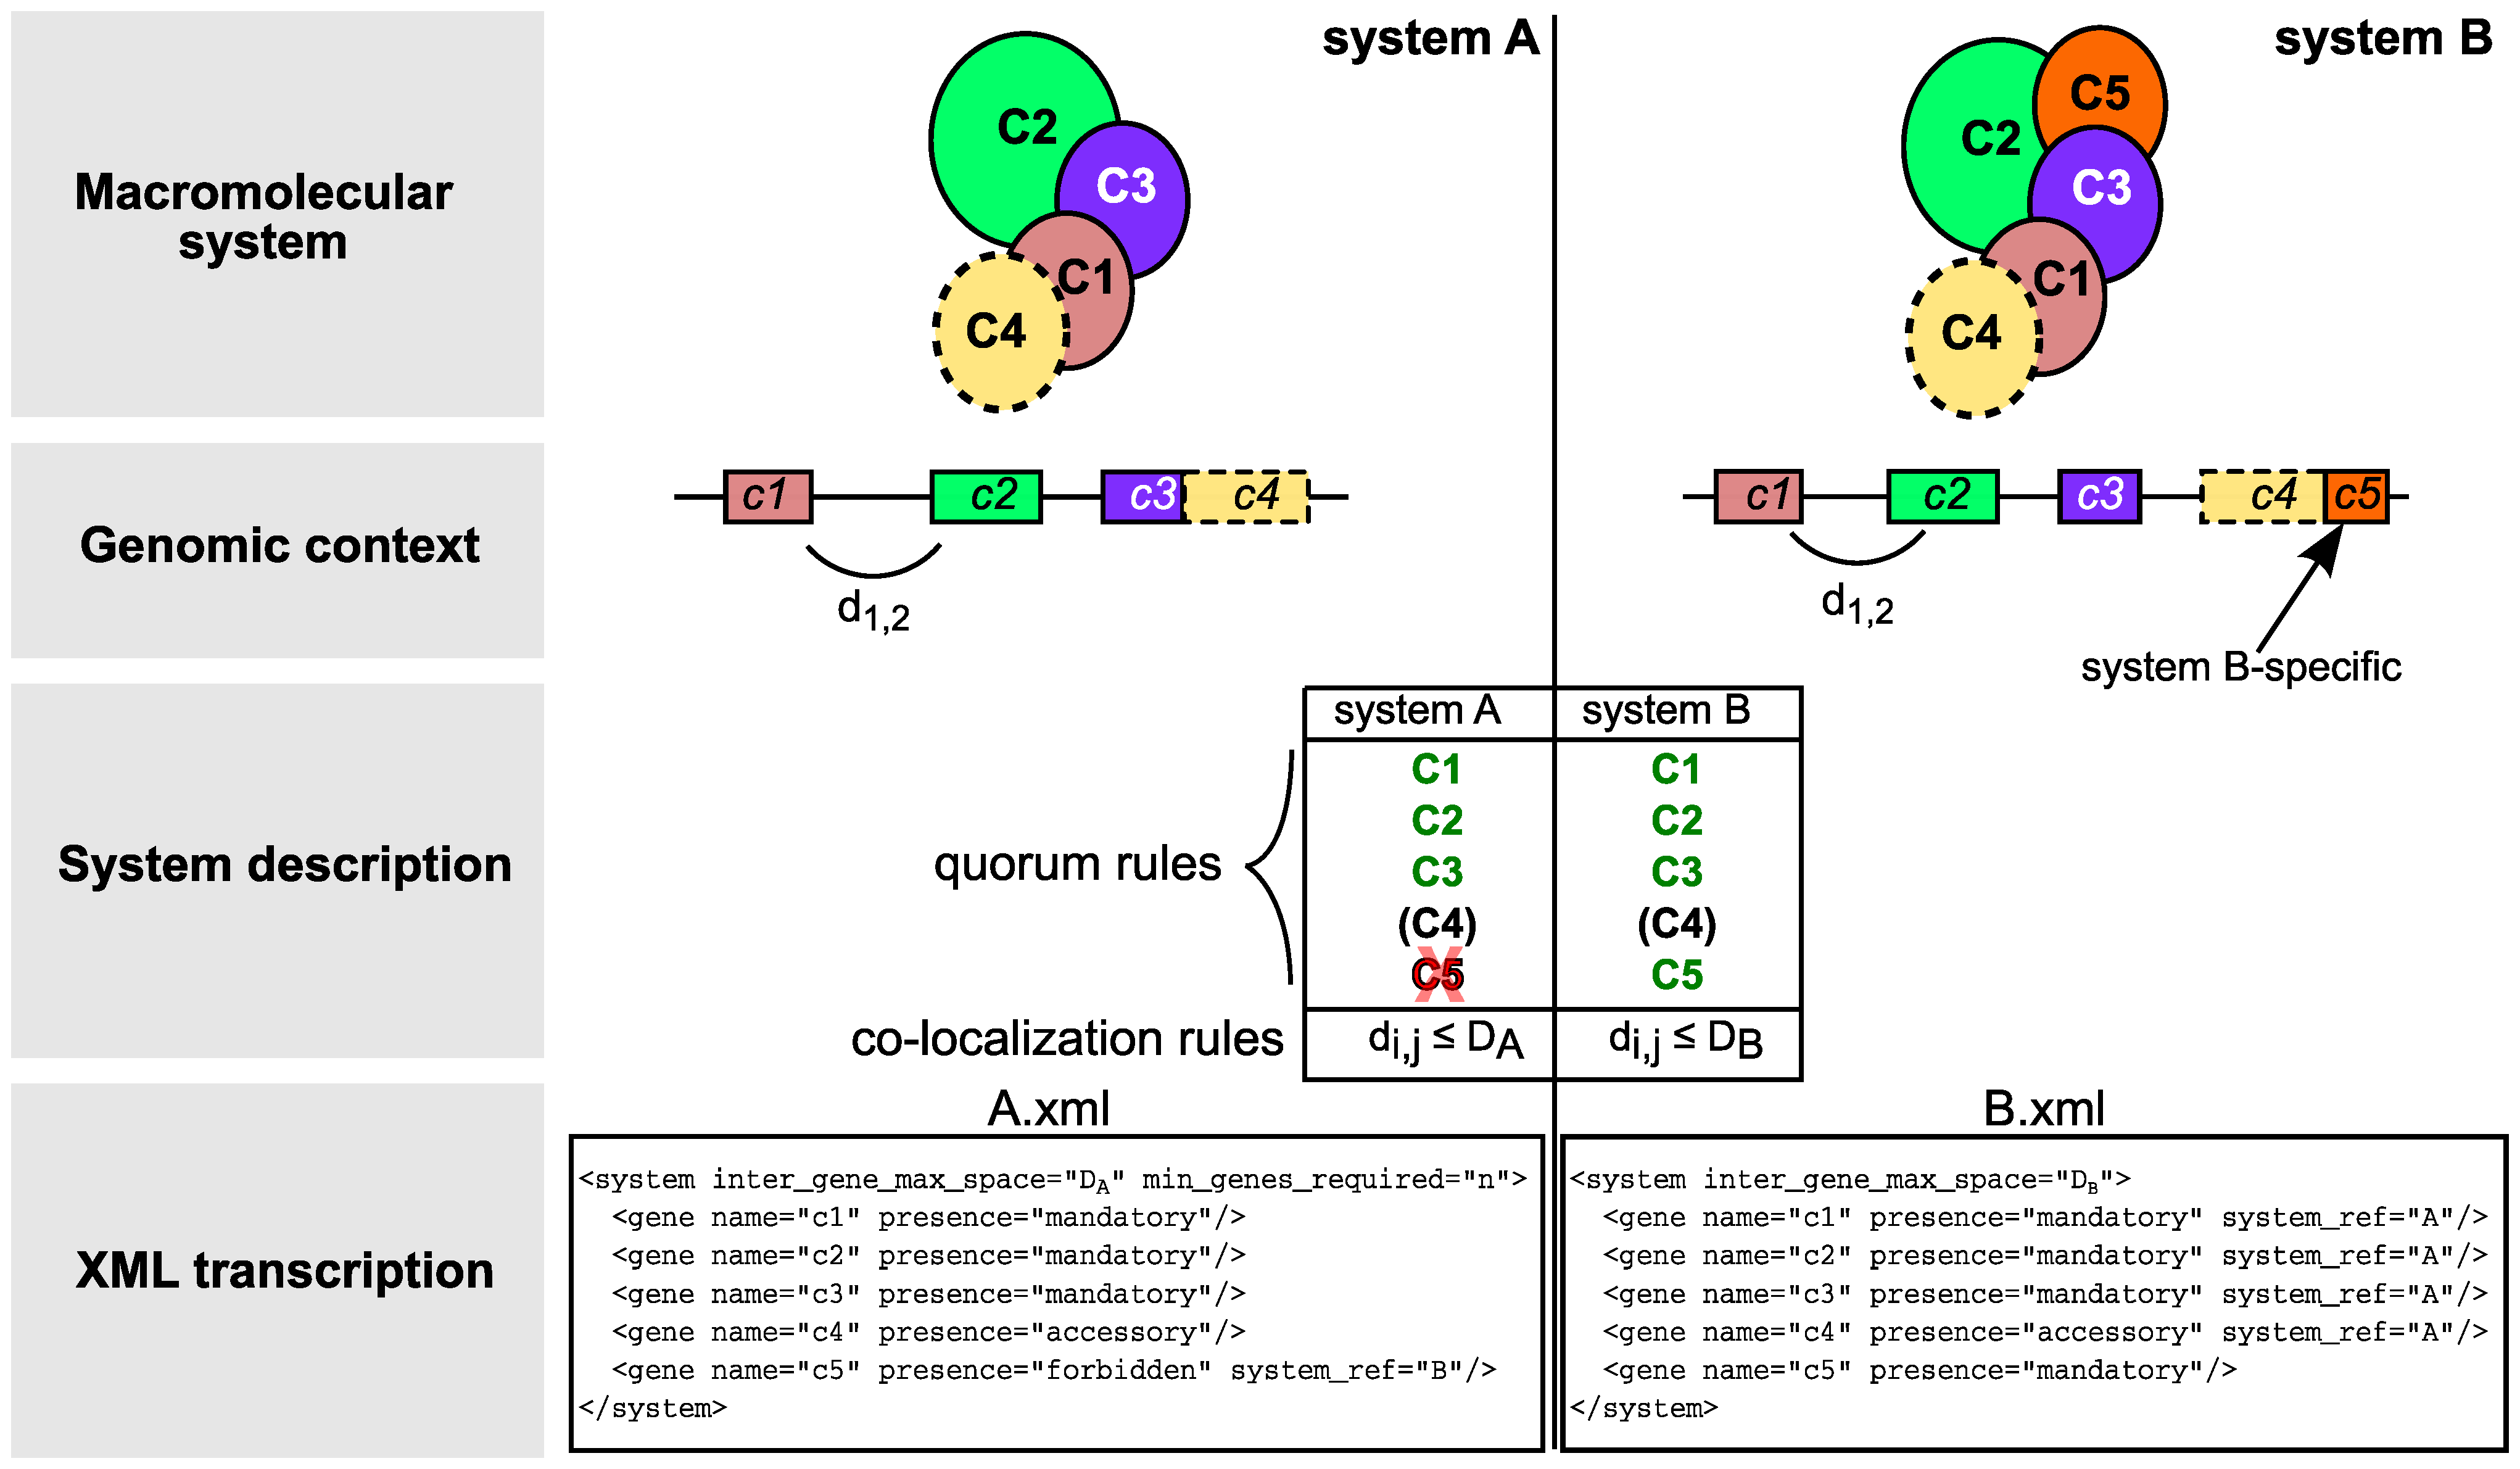
\includegraphics[width=\linewidth]{images/macsyfinder.png}
    \caption[Exemple de modélisation de systèmes dans MacSyFinder]{\textbf{Exemple de modélisation de systèmes dans MacSyFinder.} Extrait de \cite{abby_macsyfinder_2014}}
    \label{fig:macsyfinder}
\end{figure}

Plus récemment, T4SEpre \cite{wang_prediction_2014} et T4SEpp \cite{hu_t4sepp_2024} ont utilisé des modèles et des méthodes d'apprentissage automatique pour améliorer la sensibilité et la spécificité de la prédiction des systèmes T4SS.

\paragraph{Systèmes impliqués dans le métabolisme secondaire}

En 2011, antiSMASH \cite{medema_antismash_2011} a marqué une avancée majeure en automatisant l'identification des groupes de gènes colocalisés impliqués dans une voie de biosynthèse, appelés \textit{Biosynthetic Gene Clusters} (BGCs). Cette identification repose sur une vaste base de données de profils HMM, permettant la détection d'un large éventail de BGCs, notamment les NRPS (peptides non ribosomiques), les PKS (polykétides), les RIPP (\textit{Ribosomally Synthesized and Post-translationally Modified Peptides}) ainsi que d'autres métabolites secondaires.

Des méthodes récentes, telles que DeepBGC \cite{hannigan_deep_2019} et GECCO \cite{carroll_accurate_2021}, utilisent des modèles de \textit{deep learning} et des approches de traitement du langage naturel pour prédire les BGCs. Ces méthodes permettent une classification plus précise, bien qu'elles nécessitent une puissance de calcul importante et soient moins accessibles aux microbiologistes que les outils classiques.

\newpage

\subsection{Les systèmes de défense aux phages}
\label{sec:def}

Dans leur environnement naturel, les procaryotes sont fréquemment exposées à l’infection par des \textbf{phages}. Au fil de l’évolution, ces virus ont développé une remarquable diversité de mécanismes leur permettant d’infecter un éventail plus ou moins large d’espèces. Ces dernières années, l’intérêt pour les phages s’est considérablement accru, passant de 452 publications mentionnant le terme phage dans les MeSH Terms de PubMed en 2000 à 1250 en 2024. Cet engouement est notamment porté par la reconsidération de la \textbf{phagothérapie}\footnote{Utilisation des phages pour traiter certaines maladies en ciblant sélectivement les cellules.}, une approche permettant de combattre les infections bactériennes \cite{boniver_phage_2022}. Bien que cette stratégie thérapeutique ait été utilisée dès l’après Première Guerre mondiale, elle a progressivement été délaissée au profit des antibiotiques. Toutefois, la montée alarmante des souches bactériennes multirésistantes conduit aujourd’hui à réexaminer les phages comme une alternative thérapeutique.

Face à ces infections, les procaryotes ont, eux aussi, développé une vaste panoplie de mécanismes regroupés sous le terme \textbf{systèmes de défense contre les phages}. Cette compétition entraîne une course coévolutive, menant à une diversification continue des stratégies d’infection des phages et des systèmes de défense. Les microbiologistes s’intéressent de plus en plus à ces interactions complexes, non seulement pour leurs applications pratiques en génétique moléculaire, comme l’exploitation des enzymes de restriction, mais aussi pour leur potentiel dans le développement de la phagothérapie. La connaissance des mécanismes permettant à une souche de résister à une gamme spécifique de phages étant essentielle pour concevoir des traitements efficaces et adaptés.

\subsubsection{Phages : retour sur les virus de bactéries}
\label{sec:phage}
Les virus infectant les bactéries, connus sous le nom de bactériophages ou phages, ont été observés pour la première fois en 1915 et décrits officiellement par Félix d'Hérelle. Ces phages, dont la taille varie entre 20 et 200 nanomètres, présentent une grande diversité de formes. Leur matériel génétique peut être constitué d'ADN ou d'ARN, en simple ou double brin (\autoref{fig:phages}). Chaque phage possède un spectre d'hôtes spécifique, \textit{i.e}, qu'il ne peut infecter qu'un nombre restreint et défini d'espèces procaryotes.

\begin{figure}[htbp]
    \centering
    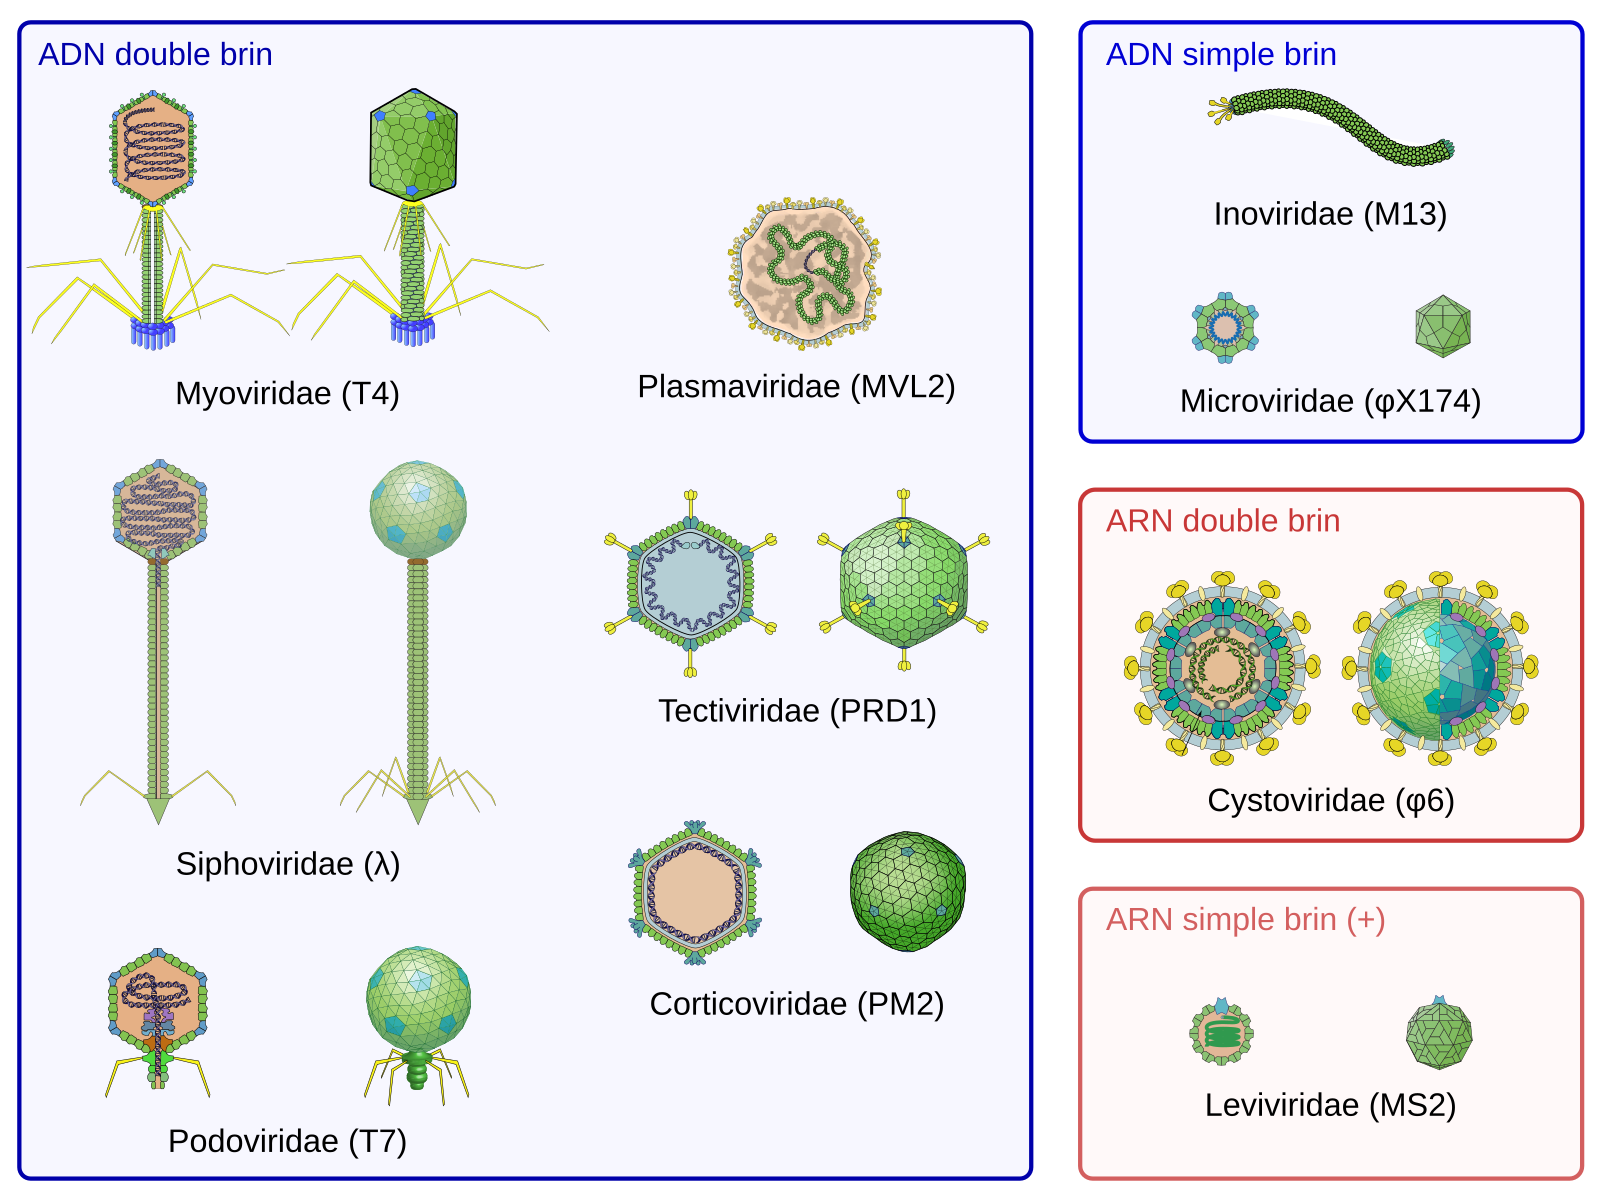
\includegraphics[width=0.75\linewidth]{images/phages.png}
    \caption[Diversité morphologique parmi les phages]{Diversité morphologique des phages. Auteur : Philippe Le Mercier - ViralZone SIB Swiss Institute of Bioinformatics}
    \label{fig:phages}
\end{figure}

Les phages ne sont pas capables de répliquer leur propre matériel génétique, c'est pourquoi ils infectent les cellules procaryotes, afin d'utiliser les systèmes de réplication de l'hôte. Une fois que le matériel a été répliqué (des milliers de fois), les nouveaux phages seront libérés dans l'environnement en lysant la cellule (ouverture de la paroi). Le cycle d'infection, réplication, libération existe sous 2 formes définissant 2 catégories de phages (\autoref{fig:cycle_phage}). Le cycle lytique, réalisé par les phages virulents, correspond à un cycle court où le phage détruit l'hôte à la fin de sa réplication. Le cycle lysogénique, opéré par les phages tempérés, réfère à un phage qui va rester dans la cellule pendant plusieurs cycles de réplication de l'hôte. Dans ce cas, le matériel génétique peut s'intégrer au chromosome de l'hôte et se répliquer avec lui, on parle de région prophagique, ou rester dans le cytoplasme sous forme d'épisome et se répliquer indépendamment comme un plasmide.

\begin{figure}
    \centering
    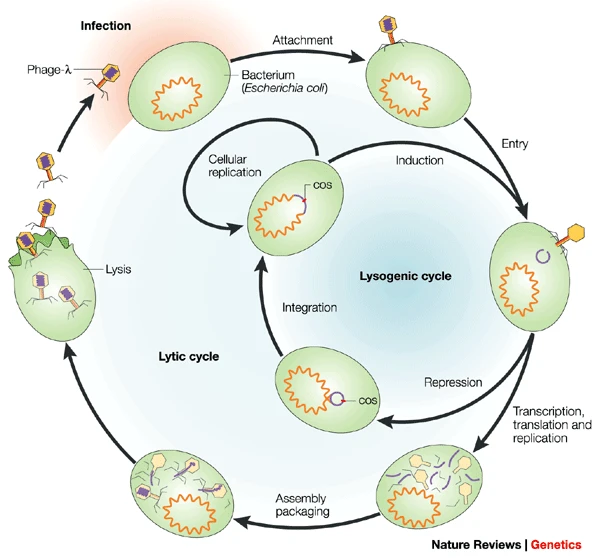
\includegraphics[width=0.75\linewidth]{images/cycle_phages.png}
    \caption[Cycle de vie des phages]{Cycle de vie des phages. Extrait de \cite{campbell_future_2003}}
    \label{fig:cycle_phage}
\end{figure}

\newpage
\subsubsection{Mécanismes de défense contre les phages}

Pour se défendre contre les phages, les procaryotes ont  développé un arsenal pour se protéger : les systèmes de défense contre les phages\footnote{que nous raccourcirons en systèmes de défense dans cette partie} \cite{makarova_comparative_2013}. Un système de défense correspond à un ensemble de protéines qui vont empêcher l'infection du phage et donc empêcher la destruction de la cellule. Ils peuvent agir de manière très diverse et à différent moment du cycle de vie du phage. 

%Dans la nature, il en existe une grande diversité et un organisme n'est capable d'en utiliser seulement une partie. 

Les premiers systèmes de défense ont été identifiés dans les années 50, il s'agit des systèmes de restriction-modification (RM) \cite{bertani_host_1953}. Ces systèmes sont composés de deux fonctions principales, généralement assurées par deux protéines distinctes : la reconnaissance et la coupure de l'ADN étranger (REase), et la modification par méthylation (MTase) pour protéger l'ADN de la coupure. La REase n'étant pas spécifique, l'action de la MTase permet de prévenir et de protéger les réplicons de l'hôte contre les coupures.

C'est à partir des années 2000 que de nouveaux systèmes de défense ont été identifiés. Les systèmes CRISPR-Cas, connus notamment aujourd'hui pour leur application en médecine et en génétique en tant que ciseaux moléculaires\cite{haft_guild_2005,barrangou_crispr_2007}\footnote{Emmanuelle Charpentier et Jennifer A. Doudna ont reçu le prix Nobel de chimie en 2020 pour avoir découvert les ciseaux génétiques CRISPR/Cas9} pour découper des séquences d'ADN cible. Les CRISPRs correspondent à des clusters de séquences palindromiques répétés et régulièrement espacés par des régions appelées \textit{spacer}. Les séquences CRISPR sont associées à des protéines Cas dont la première fonction est de se lier à des transcrits de \textit{spacer} pour identifier spécifiquement l'ADN étranger dans la cellule et de le découper. La seconde fonction va être de récupérer cet ADN pour l'intégrer dans le chromosome entre des séquences CRISPR et en faire un nouveau \textit{spacer}. Certains de ces \textit{spacers} correspondent à des séquences d'ADN phagique et seront utilisés par des protéines Cas pour combattre l'infection virale. Les systèmes CRISPR-Cas permettent donc à la cellule de répondre efficacement aux infections par des phages connus, mais aussi de construire une mémoire des infections phagiques.

Il existe également des systèmes d'infection abortive (Abi, pour \textit{Abortive infection} en anglais) qui entraînent la mort de l'hôte avant la réplication du phage \cite{molineux_host-parasite_1991}. Contrairement aux mécanismes précédents qui protègent l'hôte de l'infection, ces mécanismes permettent de protéger les bactéries environnantes en empêchant le phage de se multiplier. Récemment, la découverte récente de nouveaux systèmes Abi a mené à revoir leur définition et leur classification en tant que mécanisme de défense est discuté. Dans leur article, Aframian et Eldar soutiennent que Abi ne doit pas être considéré comme un système de défense, mais comme une issue possible pour l'organisme, qu'il peut emprunter dans certaines conditions \cite{aframian_abortive_2023}.

Aujourd'hui, plus de 150 systèmes sont référencés et pour la majorité, ils ont été découverts dans les 10 dernières années, suite à l'intérêt croissant pour les phages et leur application, mais aussi au développement de méthodes pour les détecter. En 2018, Doron, Melamed \textit{et al.} \cite{doron_systematic_2018} ont étudié les gènes localisés à proximité de systèmes de défense. Les systèmes de défense étant concentrés dans les îlots génomiques (îlots de défense)\cite{makarova_defense_2011}, ils ont spécifiquement étudié ces régions. Ils ont ainsi pu identifier 26 nouveaux systèmes de défense, dont 9 qui ont pu être confirmés expérimentalement. Les études suivantes, qui ont permis d'identifier de nouveaux systèmes, se basent sur la même stratégie.

Les systèmes de défense peuvent être classés en 3 grandes catégories (\autoref{fig:defsys}) :
\begin{enumerate}[label=(\roman*)]
    \item Les systèmes qui reconnaissent l'ADN des phages, utilisent des séquences d'ADN pour identifier et dégrader l'ADN viral, offrant ainsi une immunité adaptative;
    \item Les systèmes qui reconnaissent les protéines de phages, tels que les systèmes AVAST \cite{gao_diverse_2020}, ciblent et inactivent les protéines essentielles des phages, empêchant ainsi leur réplication;
    \item les systèmes surveillant l'intégrité de la cellule, comme le système toxine-antitoxine : ToxIN \cite{guegler_shutoff_2021}, déclenchent des réponses suicidaires ou de dormance cellulaire en réponse à des dommages ou stress induits par les phages, limitant ainsi la propagation de l'infection.
\end{enumerate}

D’autres systèmes, bien que moins caractérisés, jouent un rôle tout aussi important, incluent des mécanismes diversifiés qui interfèrent avec différentes étapes du cycle de vie des phages. Par exemple, le système CBASS (Cyclic oligonucleotide-Based Anti-phage Signaling System), déclenche une réponse suicidaire contrôlée en cas d'infection virale, empêchant ainsi la propagation du phage. Un autre exemple est celui des systèmes viperin\footnote{Système homologue à celui des eucaryotes}, inhibent la réplication virale en produisant des analogues de nucléotides modifiés qui bloquent la transcription de l'ADN phagique en agissant comme des chaînes de terminaison précoce. Ces stratégies contribuent à la résistance bactérienne globale contre les infections virales.

\begin{figure}[htbp]
    \centering
    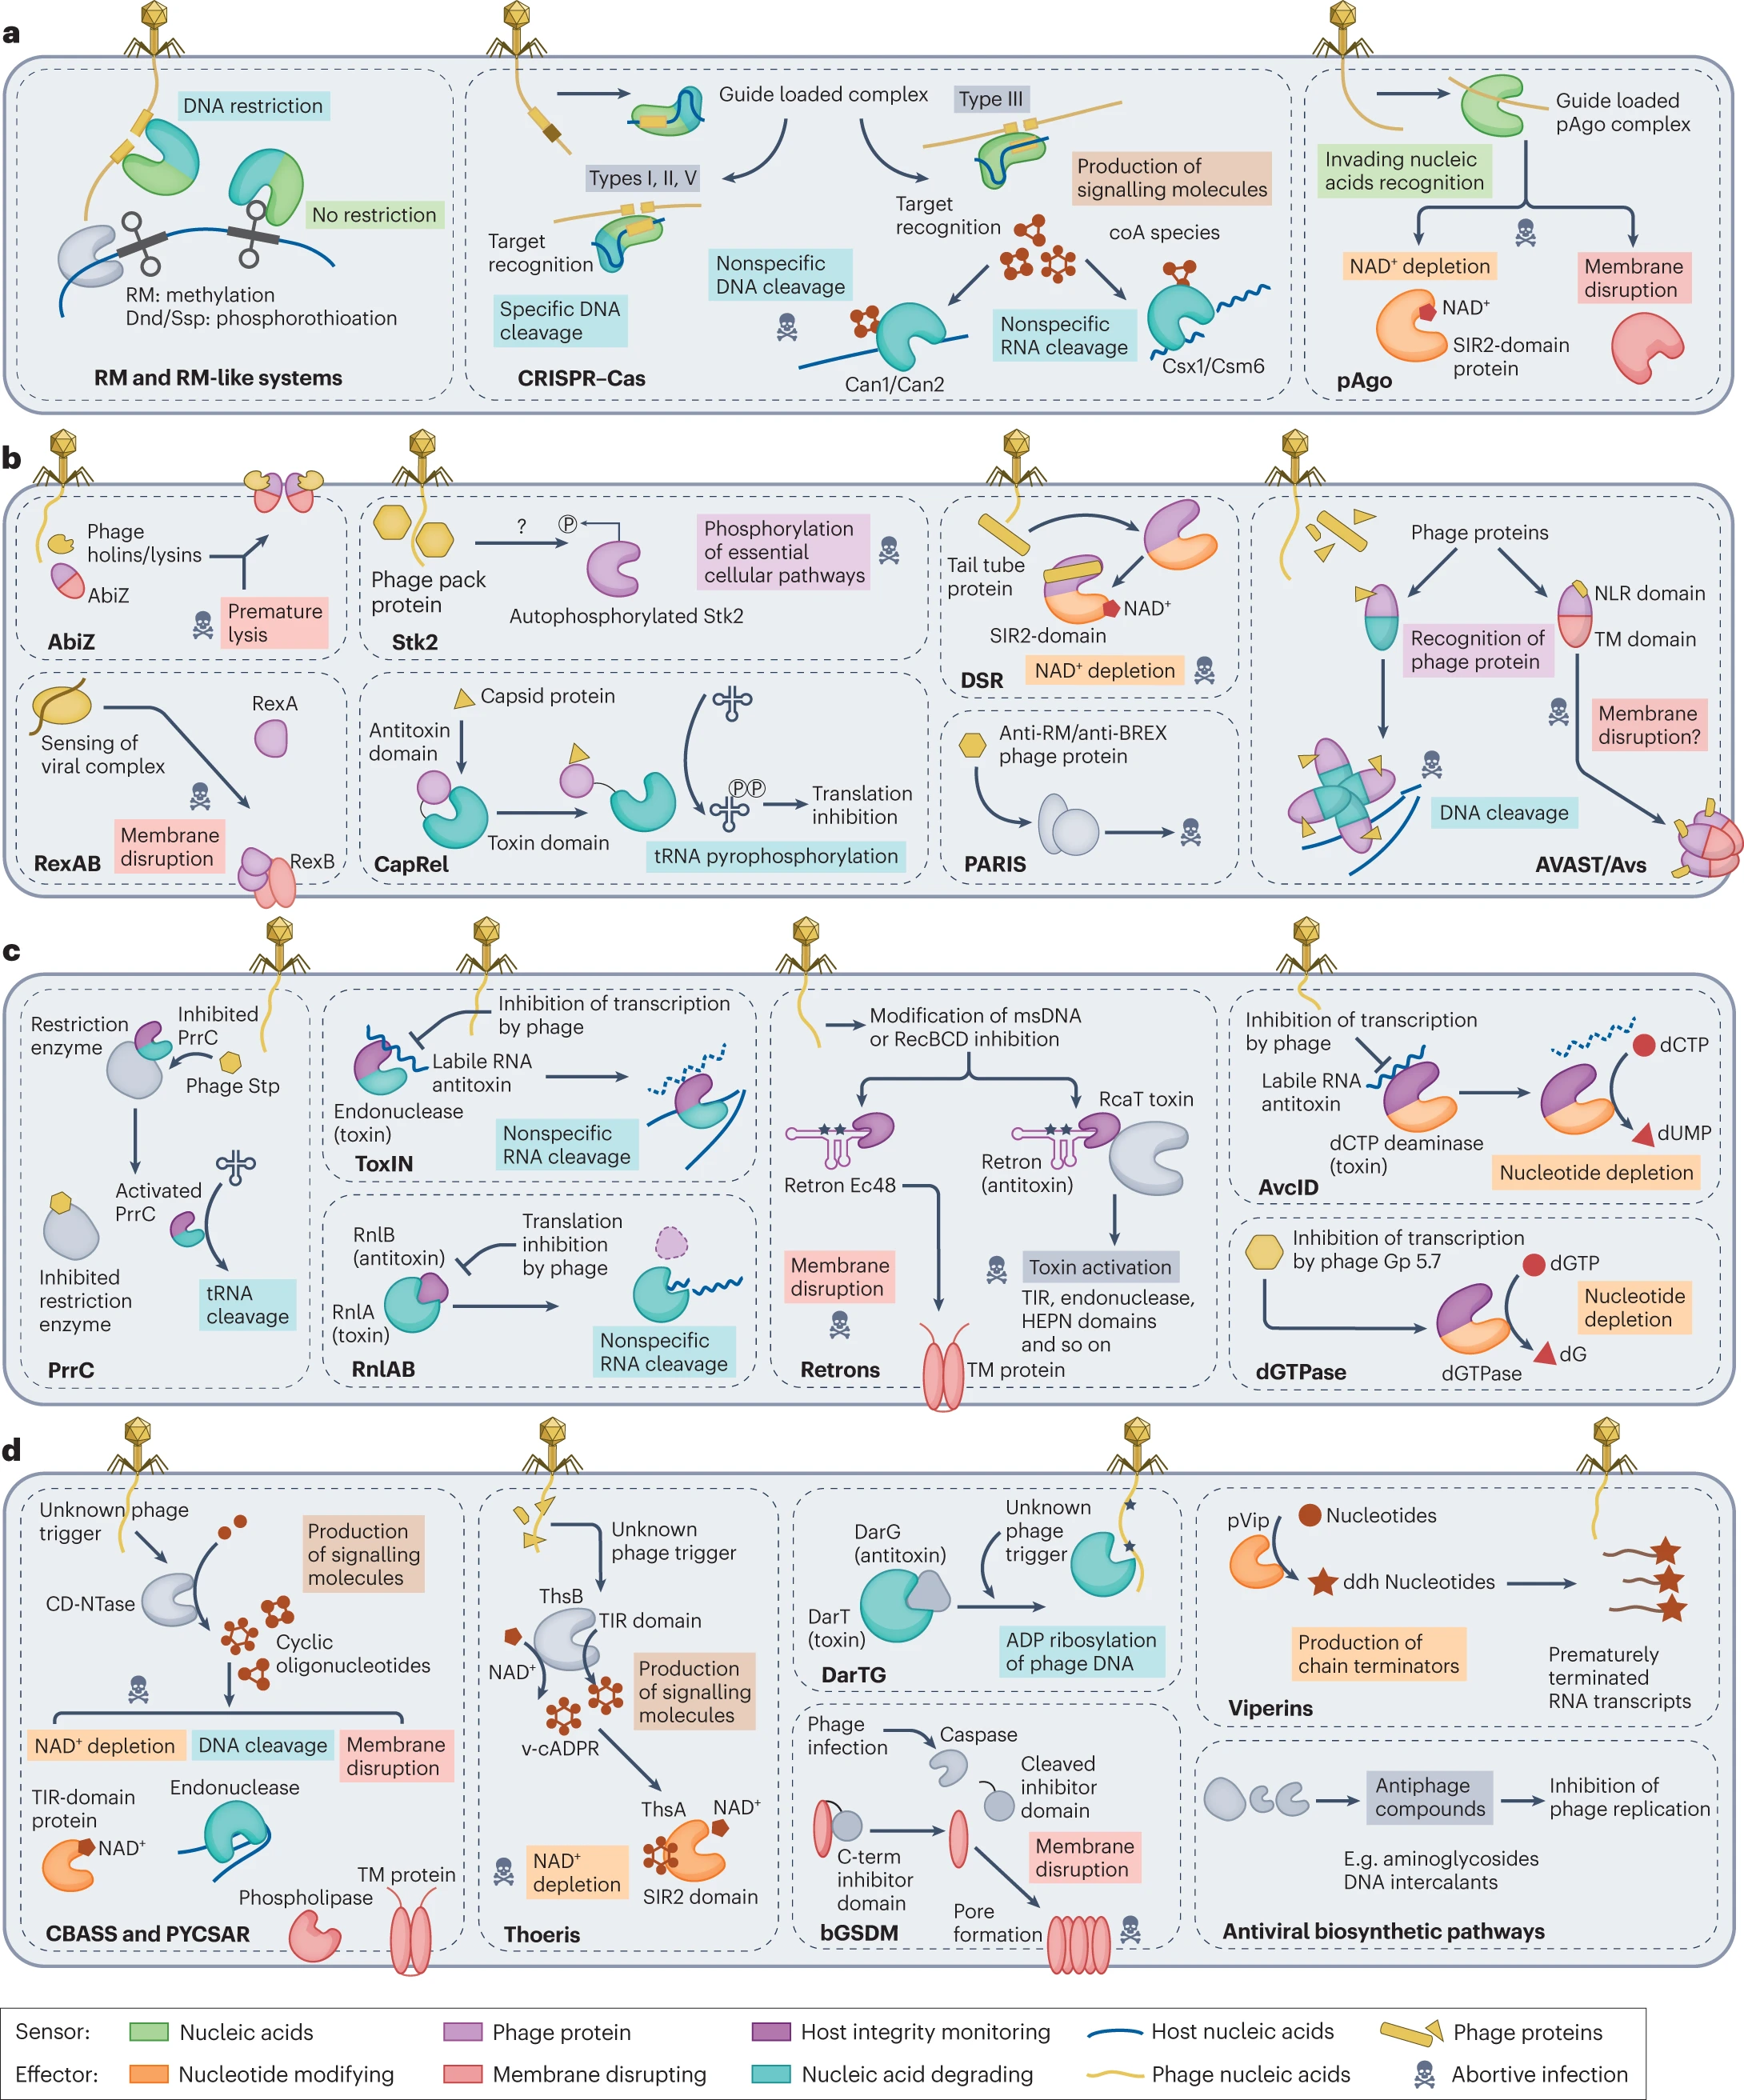
\includegraphics[width=\textwidth]{images/defensesys.png}
    \caption[Diversité des systèmes de défenses aux phages]{\textbf{Diversité des systèmes de défenses aux phages.} \textbf{a}) Systèmes de détection d'ADN étranger. \textbf{b}) Systèmes sensibles aux protéines phagiques. \textbf{c}) Systèmes de surveillance de l'intégrité de l'hôte. \textbf{d}) Autres mécanismes.  Extrait de \cite{georjon_highly_2023}}
    \label{fig:defsys}
\end{figure}

\newpage

Dans le même temps, avec l'émergence d'outils de détection (cf. \autoref{sec:defmet}), on s'intéresse à la distribution de ces systèmes dans les espèces procaryotes. Bernheim et Sorek \cite{bernheim_pan-immune_2020} ont montré qu'au sein d'une espèce toutes les souches ne présentent pas les mêmes systèmes et que les organismes s'échangent des systèmes par transfert horizontal. Cette propriété permet aux organismes de rapidement s'adapter aux phages présents dans l'environnement. Le système immunitaire doit donc être considéré comme l'ensemble des systèmes présents dans les organismes de l'environnement. En 2022, Tesson \textit{et al.} a montré que la composition en systèmes de défense varie entre les espèces, mais aussi selon la taille du génome, le risque d'infection et le mode de vie \cite{tesson_systematic_2022}. La composition en systèmes de défense est aussi étroitement liée aux phages qui peuvent infecter la bactérie, et réciproquement \cite{srikant_evolution_2022}. Pour terminer, Beavogui \textit{et al.} se sont intéressés au système immunitaire dans les données de génomique environnementale et ont montré une distribution différente des systèmes de défense en fonction de l'habitat et de la géographie \cite{beavogui_defensome_2024}.

Toutes ces études ont été permises par l'arrivée de méthodes et d'outils de détection automatique des systèmes de défense dans les génomes.

\subsubsection{Méthodes et outils de détection}
\label{sec:defmet}

Les premiers outils de détection dans les génomes, étaient spécialisés dans l'identification des systèmes CRISPR. Leur approche reposait sur la recherche de séquences répétées intercalées de séquences uniques, grâce à des méthodes d’alignement. PILER-CR \cite{edgar_piler-cr_2007} identifie d'abord toutes les séquences répétées palindromiques, sélectionne celles correspondant aux CRISPR (24 à 48 pb, séparées par des séquences uniques), puis affine leur détection grâce à une approche basée sur l’analyse de graphes et le partitionnement. L'outil CRT \cite{bland_crispr_2007}, utilise des k-mers pour rechercher des séquences répétées d'une taille donnée, éloignées d'une distance définie et dont la séquence est unique. Ces 2 méthodes sont rapides et ont l'intérêt de détecter toutes les séquences répétées candidates pour être des CRISPR. L'outil CRISPRFinder \cite{grissa_crisprfinder_2007}, va suivre un schéma similaire aux outils précédents, mais va introduire une notion de score, qui prend en compte le nombre de répétitions, leur taille, la régularité et la taille des espacements. De plus, une fois les séquences candidates filtrées, pour améliorer sa précision, CRISPRFinder peut comparer les candidats à sa base de données de CRISPRs validées.

Avec l'accumulation des connaissances autours des CRISPRs et des séquences environnantes qui les composent, les outils vont intégrer de nouveaux critères de détection. Des outils comme CRISPRstrand\cite{alkhnbashi_crisprstrand_2014}, CRISPRDirection\cite{biswas_accurate_2014} utilisent les séquences d'ARNcr\footnote{Les ARNcr, sont un type d'ARN contenant le transcrit d'une partie du CRISPR et le spacer. Ils sont utilisés dans la reconnaissance spécifique de l'ADN étranger.}, d'autres utilisent les séquences leader\footnote{Une séquence séparant les CRISPR des gènes codant pour les Cas.} comme CRISPRleader \cite{alkhnbashi_characterizing_2016}. La première version, MacSyFinder \cite{abby_macsyfinder_2014} intégrait une base de données HMM et de modèles CasFinder, pour identifier les protéines Cas et autres séquences connues proches pour identifier les systèmes CRISPR-Cas. En 2018, Une version hybride entre CRISPRFinder et CasFinder est proposé CRISPRCasFinder \cite{couvin_crisprcasfinder_2018}. Cet outil permet de prendre en compte la structure des CRISPR et des \textit{spacers}, ainsi que les gènes environnants, pour détecter finement les systèmes CRISPR-Cas.


En 2021, la découverte de nombreux nouveaux systèmes de défense a conduit au développement d’outils, comme PADLOC \cite{payne_identification_2021}, pour leur identification dans les génomes. PADLOC s’appuie sur une base de données HMM et de modèles décrivant les systèmes inspirés de la grammaire des modèles de MacSyFinder \cite{abby_macsyfinder_2014}. Peu après, DefenseFinder \cite{tesson_systematic_2022} a été publié, adoptant une approche méthodologique similaire reposant sur MacSyFinder pour la détection.
Bien que ces outils partagent un même principe de fonctionnement, ils diffèrent principalement dans la construction des profils HMM et dans les règles de détection des systèmes. PADLOC génère des HMMs entièrement \textit{de novo}, \textit{ie} qu'il construit sa propre base de données de profils, tandis que DefenseFinder s’appuie en partie sur des bases de données de protéines existantes, comme Pfam\cite{mistry_pfam_2021}. Par ailleurs, PADLOC privilégie une approche fondée sur des modèles plus généralistes, intégrant des règles plus flexibles afin de faciliter l’identification de systèmes proches de ceux connus. À l’inverse, DefenseFinder adopte des modèles plus stricts, intégrant un plus grand nombre de paramètres pour affiner la classification des systèmes identifiés.
Ainsi, le choix entre ces deux outils doit être guidé par les objectifs spécifiques de l’étude. PADLOC constitue une solution privilégiée pour les analyses exploratoires visant à détecter de nouveaux systèmes proches, tandis que DefenseFinder se révèle plus adapté aux études nécessitant une identification précise et rigoureuse des systèmes déjà caractérisés.